\documentclass{article}
\usepackage{geometry}  
\usepackage{amsmath}  
\usepackage{graphicx} 
\usepackage{svg}
\usepackage[T1]{fontenc}
\usepackage{float}
\usepackage[utf8]{inputenc}
\usepackage{array}
\usepackage{booktabs}
\usepackage{gensymb}
% wklejanie obrazków
%\begin{figure} [!ht]
%	\begin{center}
%			\includegraphics[width = \textwidth]{konsola_zad_1.png}
%			\caption{Wypisanie zawartości rejestru WHO\_AM\_I na konsoli semihostingu}
%	\end{center}
%\end{figure}

\title{ Laboratorium projektowania systemów elektronicznych\\ Laboratorium 4 \\} % Report title

\author{Anna \textsc{Dzieżyk}, indeks: 318506 }% Author name(s), add additional authors like: '\& James \textsc{Smith}'

\date{\today} % Date of the report
\begin{document}

\maketitle % Insert the title, author and date using the information specified above

\begin{center}
	\begin{tabular}{l r}
		Data wykonania ćwiczenia: & 30 listopada 2025 \\ % Date the experiment was performed
		Prowadzący: & dr inż. Maciej \textsc{Grzegrzółka} \\% Instructor/supervisor
        Nr projektu: & 2
	\end{tabular}
\end{center}

\section{Wybór elementów}
Wymagania projektowe konieczne do wykonania tego laboratorium, czyli symulacji i doporu elementów były poniższe:
\begin{enumerate}
    \item Wzmocnienie = 30V/V
    \item Pasmo pracy układu = 0Hz - 200kHz
    \item Zasilanie układu = +22V
    \item Zasilanie wzmacniacza = +17V 
\end{enumerate}
Reszta wymagań jest ważna do wykonania płytki. Z punktu 1. wynika, że należy użyć wzmacniacza operacyjnego. Punkt 2. i 4. zawęża obszar poszukiwać do 
wzmacniacza, który powinien przyjmować napięcie zasilania równe co najmniej 17V i o polu wzmocnienia równym co najmniej $f_t$ = 200kHz*30V/V = 6MHz. Wzmacniacz ADA4625-1 spełnia te wymagania. 
Następnie - skoro wzmacniacz powinien być zasilony napięciem +17V, a nie +22V, no to należy napięcie zasilania obniżyć, najwygodniej by było stabilizatorem napięcia. Wymagania co do tego elementu 
dyktuje napięcie, jakie stabilizator może przyjąć i jakie jest w stanie oddać, i przy jakim prądzie. Wybrano stabilizator oparty na układzie scalonym LT3063. Wytrzymuje napięcia wejściowe aż do 45V i może zapewniać prądy wyjściowe sięgające do 200mA. 
Na podstawie tych dwóch układów scalonych i z użyciem ich dokumentacji technicznych dobrano resztę elementów - czyli kondensatorów i rezystorów SMD w obudowach 0805, przedstawionych w poniższej tabeli:
\begin{table}[H]
\centering
\begin{tabular}{|c|c|c|c|c|c|}
\hline
nazwa & wartość & numer seryjny producenta & obudowa & producent & oznaczenie na schemacie \\ \hline
kondensator & 62 pF & 600F620FT250XT & 0805 & KYOCERA AVX & C1 \\ \hline
kondensator & $1.2\mu F$ & C0805C125K4RACTU & 0805 & KEMET & C2 \\ \hline
kondensator & $1.2\mu F$ & C0805C125K4RACTU & 0805 & KEMET & C4 \\ \hline
kondensator & $10\mu F$ & 0805X7R106KT1AT & 0805 & KYOCERA AVX & C3 \\ \hline
opornik & $10k\Omega$ & MCU0805MD1002BP500 & 0805 & Vishay & R1 \\ \hline
opornik & $1k\Omega$ & MCU08050E1001BP100 & 0805 & Vishay & R2 \\ \hline
opornik & $29.1k\Omega$ & RN73H2ATTD2912B25 & 0805 & KOA Speer & R3 \\ \hline
opornik & $16.5k\Omega$ & ERJ-P06F1652V & 0805 & Panasonic & R4 \\ \hline
opornik & $600\Omega$ & CRCW0805600RFKEAHP & 0805 & Vishay & R5 \\ \hline
\end{tabular}
\end{table}
\section{Przygotowanie schematu elektrycznego}
% wklejanie obrazków
\begin{figure} [H]
	\begin{center}
			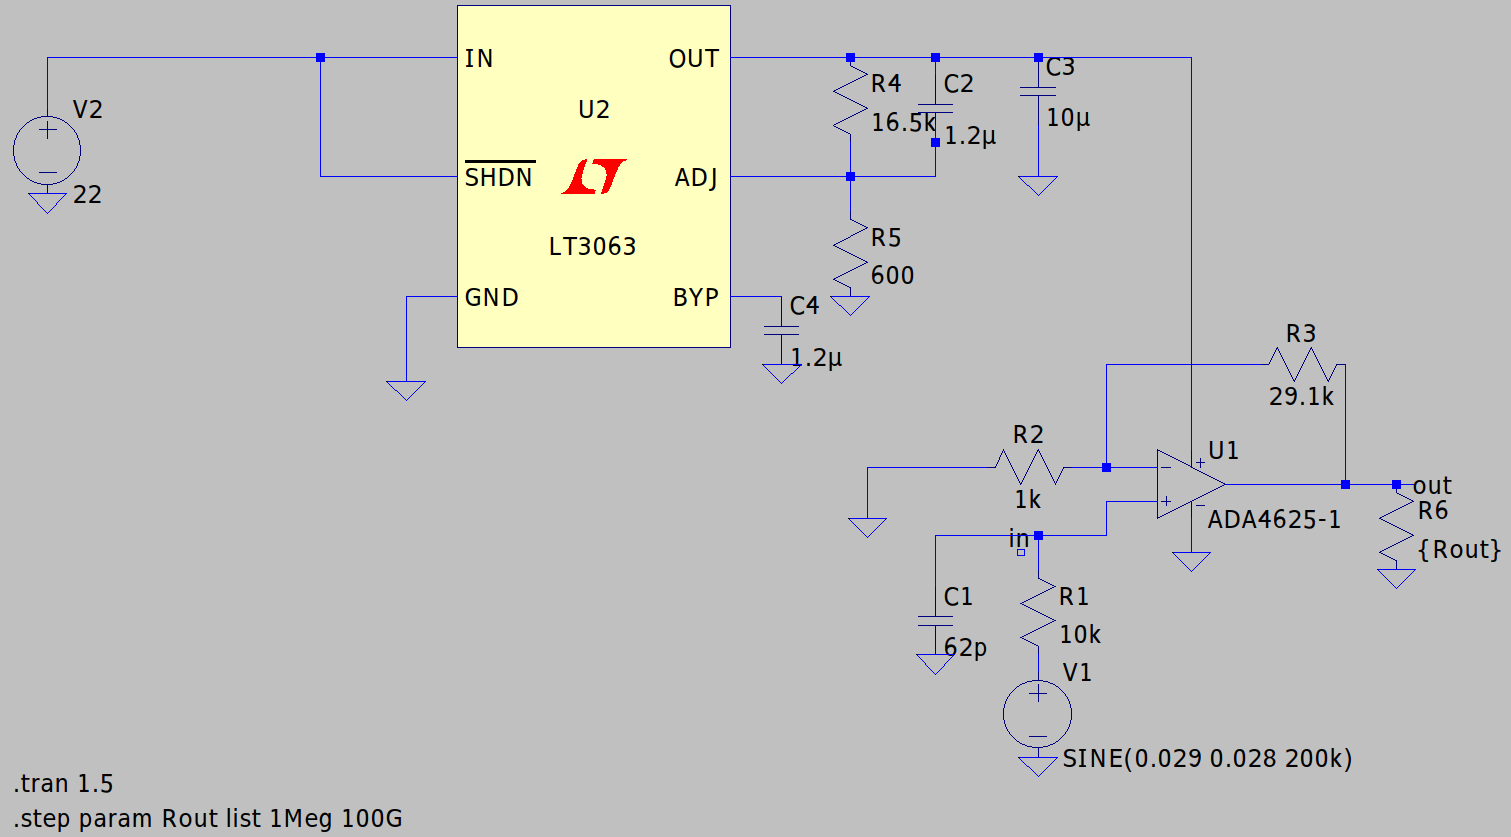
\includegraphics[width=12cm, height=5.5cm]{ss1.png}
			\caption{Schemat zaprojektowanego układu}
	\end{center}
\end{figure}
Wzmacniacz powinien być w konfiguracji nieodwracającej z pasmiem wzmocneinia do 0.2MHz = 200kHz, więc na wejściu zastosowano 
aktywny filtr dolnoprzepustowy. Wzmocnienie = 30V/V, więc wartości elementów:
\[
    \frac{R3}{R2} = 30V/V - 1 = 29
\]
Załóżmy więc, że R3 = $29,1k\Omega$ zgodnie z dostępnością elementów na stronie, a R2 = $1k\Omega$. Następnie filtr dolnoprzepustowy:
dla R1 = $10k\Omega$ C1 = 75pF i daje to częstotliowość górną równą:
\[
    f_g = \frac{1}{2*\pi*R1*C} = \frac{1}{2*\pi*10k\Omega*62pF} = 256,7kHz
\]
Jest to dosyć bezpieczny margines błędu - próg 3dB będzie niżej niż ta teoretycznie wyliczona wartość.

Dalej - elementy wokół stabilizatora. Zacznijmy od prądu - niech maksymalny prąd pobierany przez opamp będzie 
równy 1mA. Na tej podstawie - wg dokumentacji ukłądu LT3063 możemy ustalić wartości resyztorów R4 i R5 zgodnie z układem równań znależionych w dokumentacji::
\[
    I_{out} = \frac{V_{out}}{R4+R5}
\]
\[
    V_{out} = 0,6V(1+ \frac{R4}{R5}) - 15nA*R4
\]
Po szybkim rozwiąząniu układu i dostosowaniu wartości rezystorów do dostępności producentów otrzyujemy:
R4 = $16.5k\Omega$, R5 = $600\Omega$

Natomiast kondensatory zostały dobrane zgodnie z równaniem: 
\[
    C4 \geq \frac{10nF}{10\mu A} *I_{out} = \frac{10nF}{10\mu A}*1mA = 1\mu F
\]
W dokumentacji wspomniano, że najlepiej, jak C4 i C2 mają takie same wartości, więc obydwa kondensatory mają wartość $1.2\mu F$.
Ostatni kondensator został dobrany również zgodnie z sugestią z dokumentacji: C3 = $10\mu F$
\section{Symulacje}
\subsection{Symulacja transient z obciążeniem równym $1M\Omega$ i nieobciążonym układem}
\begin{figure} [H]
	\begin{center}
			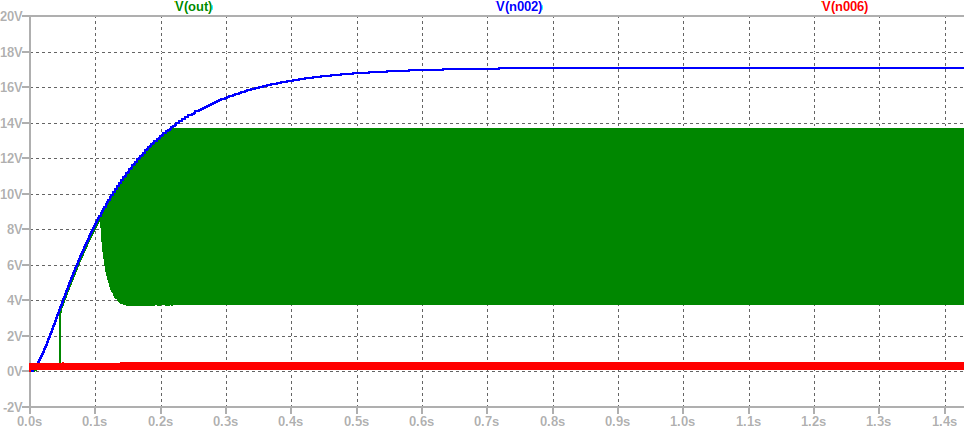
\includegraphics[width=12cm, height=5.5cm]{ss3.png}
			\caption{Wynik symulacji układu ze stabilizatorem: na tle sygnału zasilającego}
	\end{center}
\end{figure}
Sygnał ze stabilizatora jest niezakłócony, osiąga wymagany poziom po około 0.6s, jest to powolny start, ale warte zaznaczenia jest to, że poruszamy się na 
granicy częstotliwości granicznej i wzmacniamy dosyć duży i szybki sygnał wejściowy (0,321Vpp, 200kHz), który na następnym wykresie - jest niezniekształcony i nieobcięty. Układ zachowuje się identycznie
z obciążeniem nominalnym jak i bez obciążenia.
\begin{figure} [H]
	\begin{center}
			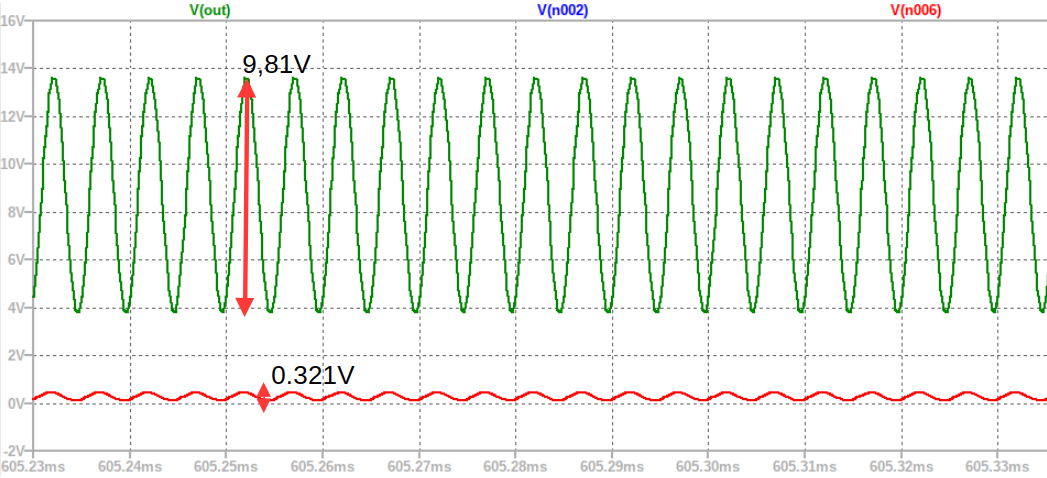
\includegraphics[width=12cm, height=5.5cm]{ss4.png}
			\caption{Wynik symulacji układu ze stabilizatorem - zbliczenie na przebiegi wejściowy i wyjściowy}
	\end{center}
\end{figure}

Wzmocnienie obliczone z danych z rysunku: k = 9,81V/0,321V = 32,5V/V - czyli spełnia wymagania. 
\subsection{Symulacje pasma częstotliwościowego}
\begin{figure} [H]
	\begin{center}
			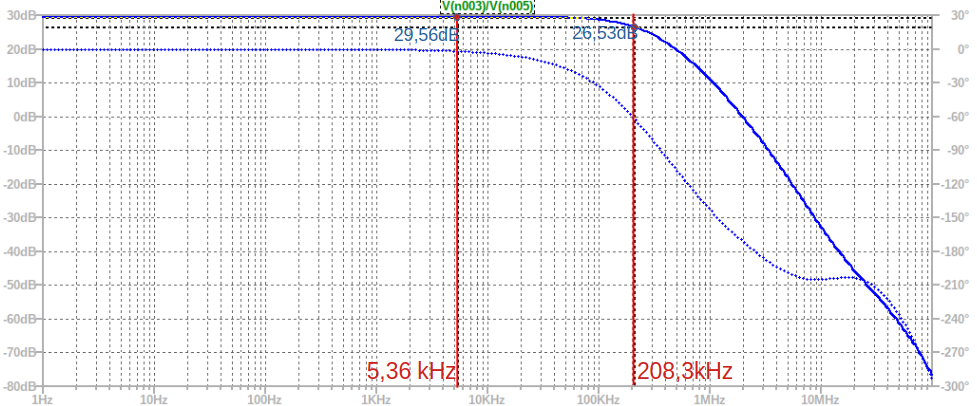
\includegraphics[width=12cm, height=5.5cm]{ss2.png}
			\caption{Wynik symulacji układu z zaznaczoną częstotliowścią spadku 3dB}
	\end{center}
\end{figure}

Pierwszą obserwacją jest to, że zachowanie układu dla obiciążenia nominalnego $1M\Omega$ jak i dla nieobciążonego jest praktycznie takie samo. Przesunięcie fazowe jest równe $0\degree$ w pasmie 
wzmocnienia. Wzmocnienie jest równe około 9.6dB w pasmie wzmocnienia, więc w skali liniowej: 
\[
    k = 10^{29.56dB/20} = 30,06V/V
\]
Co spełnia wymogi projektowe. Częstotliwość górna granczna jest równa 208,3kHz - jest to akceptowalne.
\end{document}